\section{Architecture}
\label{sec:architecture}

As this work is a blockchain-based project, the goal is to minimize the use of
traditional Web2 technologies, such as server-based backends and related
services. Instead, we aim to rely primarily on Web3 technologies to fully
understand the limitations and possibilities of adopting a blockchain-only
ecosystem. In the future, a hybrid approach combining both Web2 and Web3 could
offer significant advantages. The system architecture is depicted in Figure
\ref{fig:architecture}, illustrating how the various components of the project
interact, in line with the requirements discussed in previous sections.

\begin{figure}[H]
    \centering
    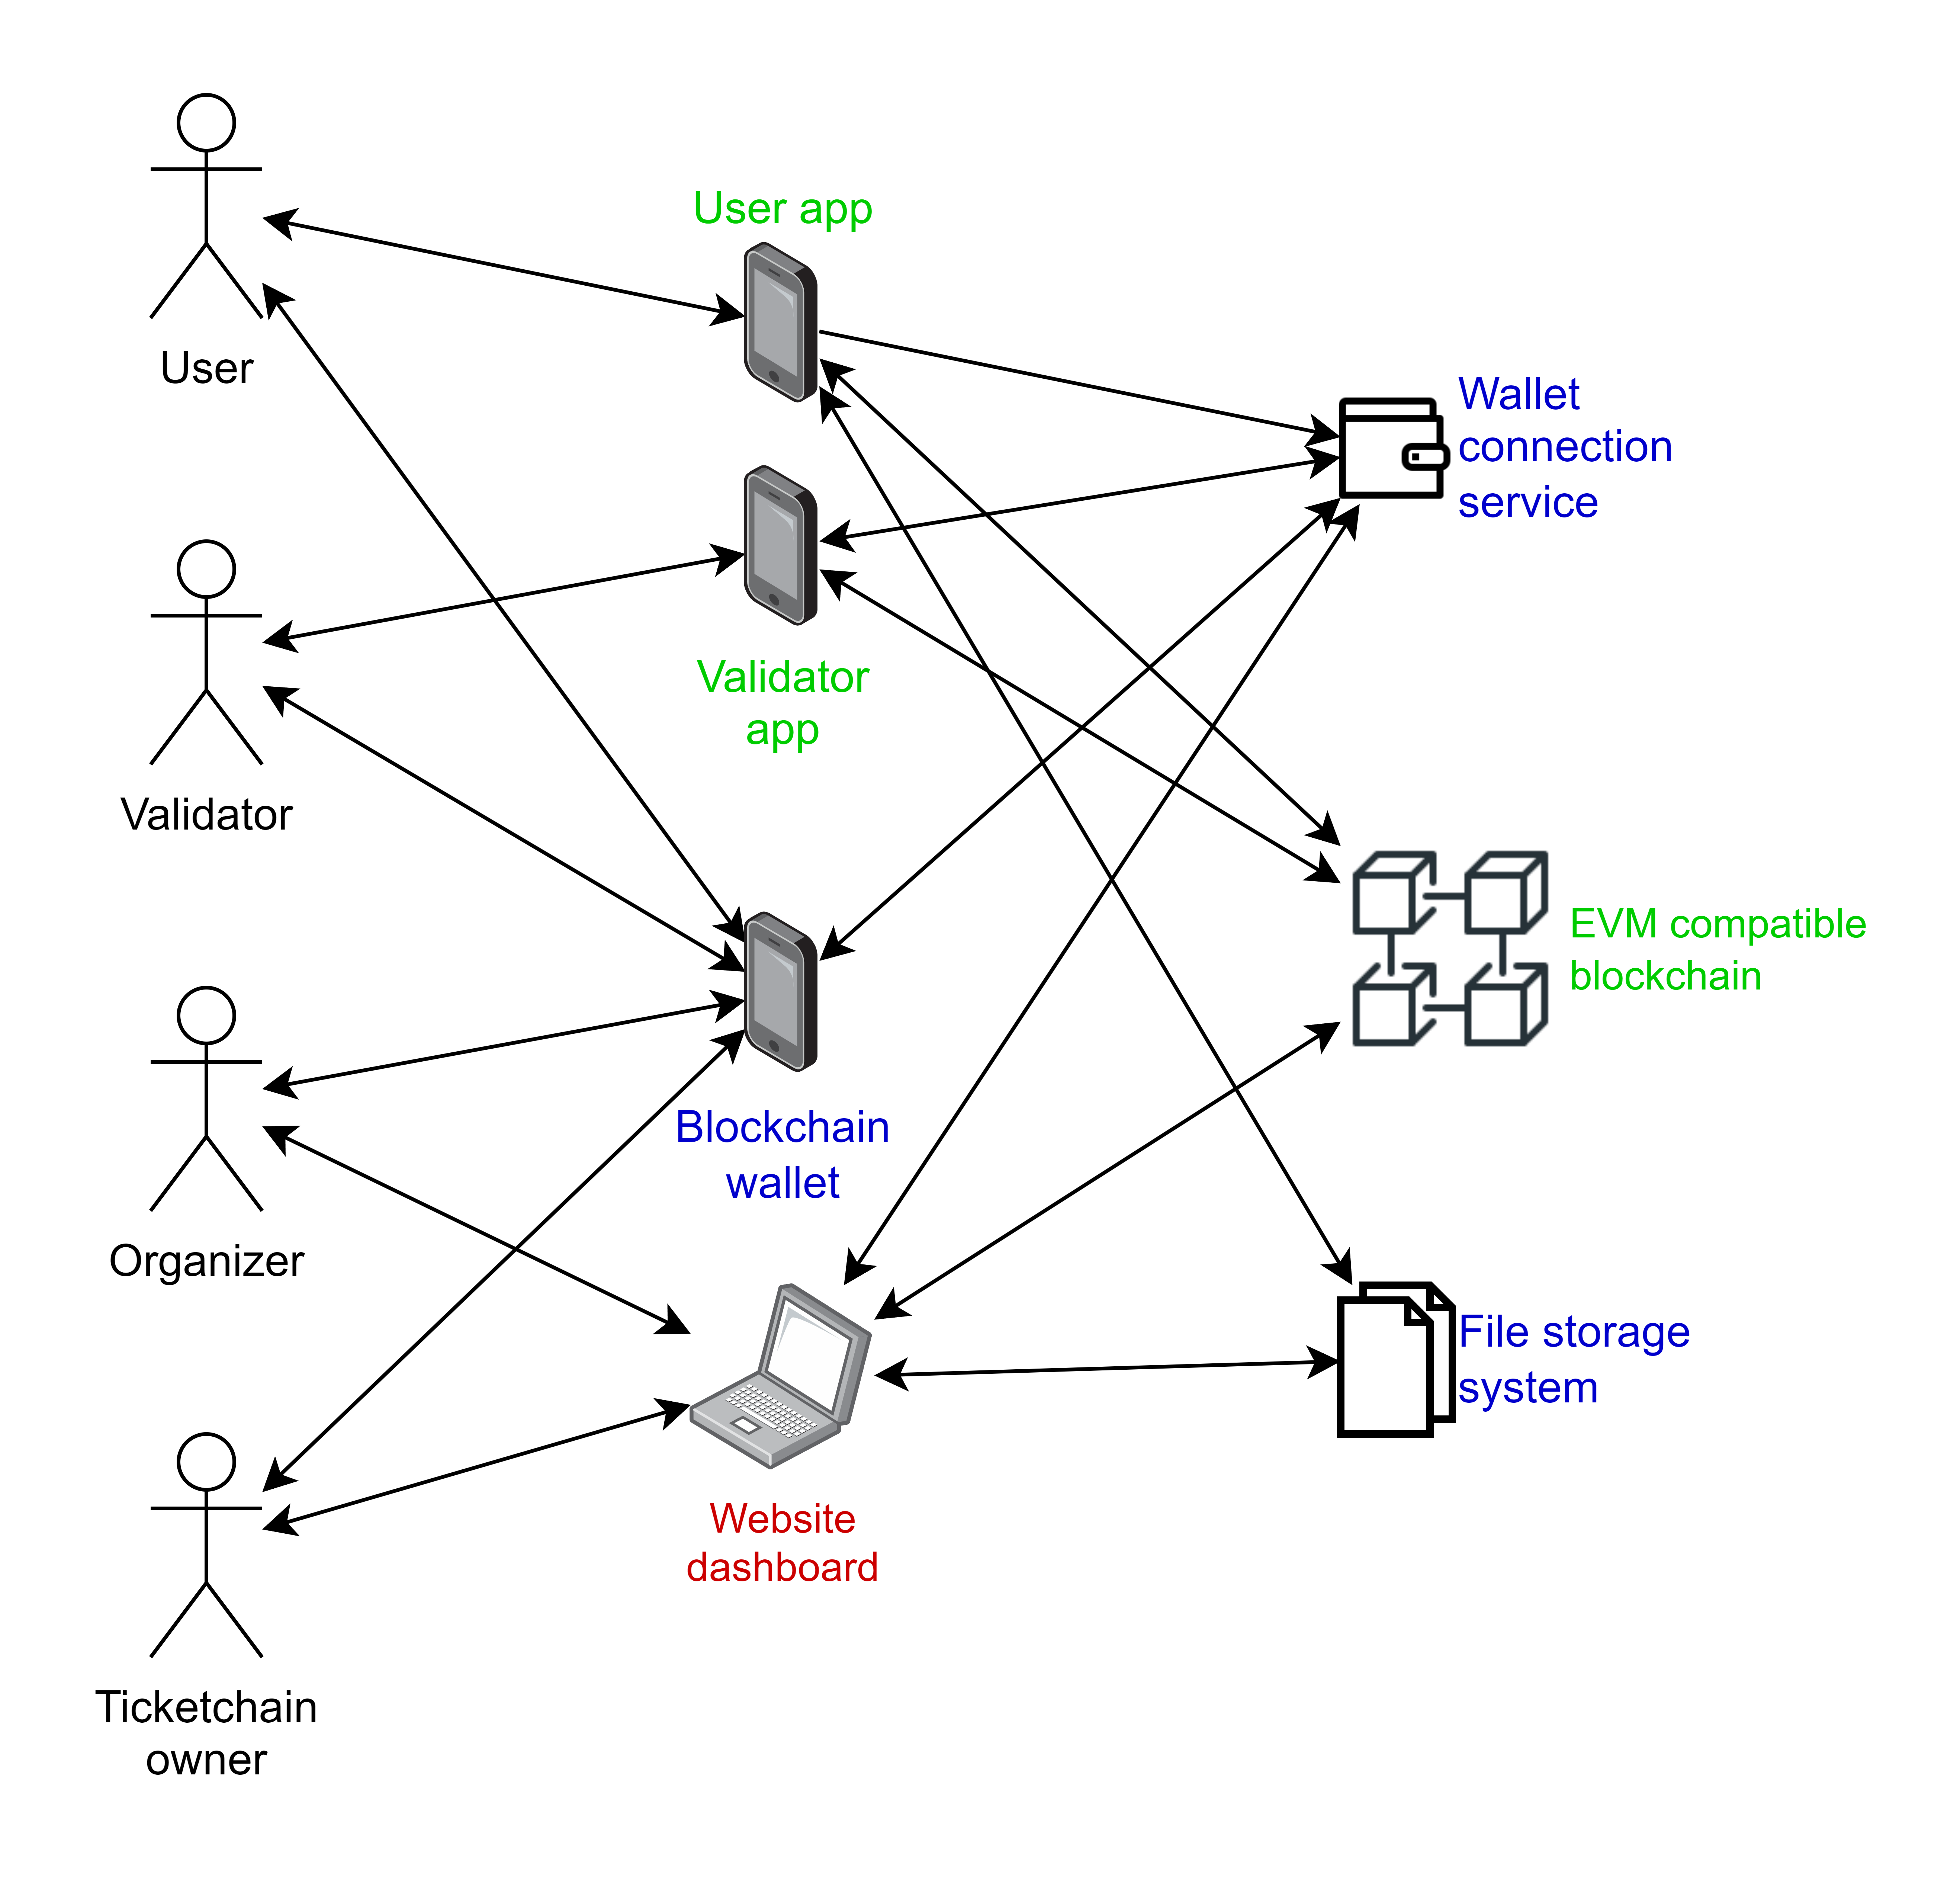
\includegraphics[width=\textwidth*2/3]{Architecture.png}
    \caption{System Architecture}
    \label{fig:architecture}
\end{figure}

The architecture includes two main mobile applications—one for regular users
and the other for validators—as well as a website dashboard for the Ticketchain
owner and event organizers to manage system settings and events.

The components highlighted in blue represent external services, while green
components denote those we are developing in the context of this project. The
red component, the website dashboard, has not yet been implemented due to time
constraints, so for now, interactions will occur directly with the smart
contract. Additionally, to streamline development, the two mobile applications
have been consolidated into a single app, allowing us to focus on the core
functionality.

As described in previous sections, all users must authenticate before accessing
the system. Instead of traditional email and password logins, authentication
will require wallet software to interact with the blockchain. Thus, a wallet
connection service is needed to link user wallets to the system.

Once authenticated, the system will interact with the smart contract to display
event-related information and update the status of events or tickets. The smart
contracts will be deployed on an EVM-compatible blockchain.

Regarding ticket images, a file storage system will be required. This serves to
store images associated to the tickets, because storing them on-chain is
expensive. Although image uploads will eventually be handled via the dashboard,
this feature is not yet implemented, necessitating manual uploads for now.
